\documentclass[11pt,a4paper,oneside]{article}
\usepackage[UTF8,adobefonts]{ctex}

\usepackage{wrapfig}
\usepackage{indentfirst}
\usepackage{amsmath}
\usepackage{float}
\usepackage{ulem}
\usepackage[top=1in,bottom=1in,left=1.25in,right=1.25in]{geometry}

\usepackage{color}
\usepackage{xcolor}

\usepackage{multirow}

\begin{document}

\begin{figure}[H]
 \centering
  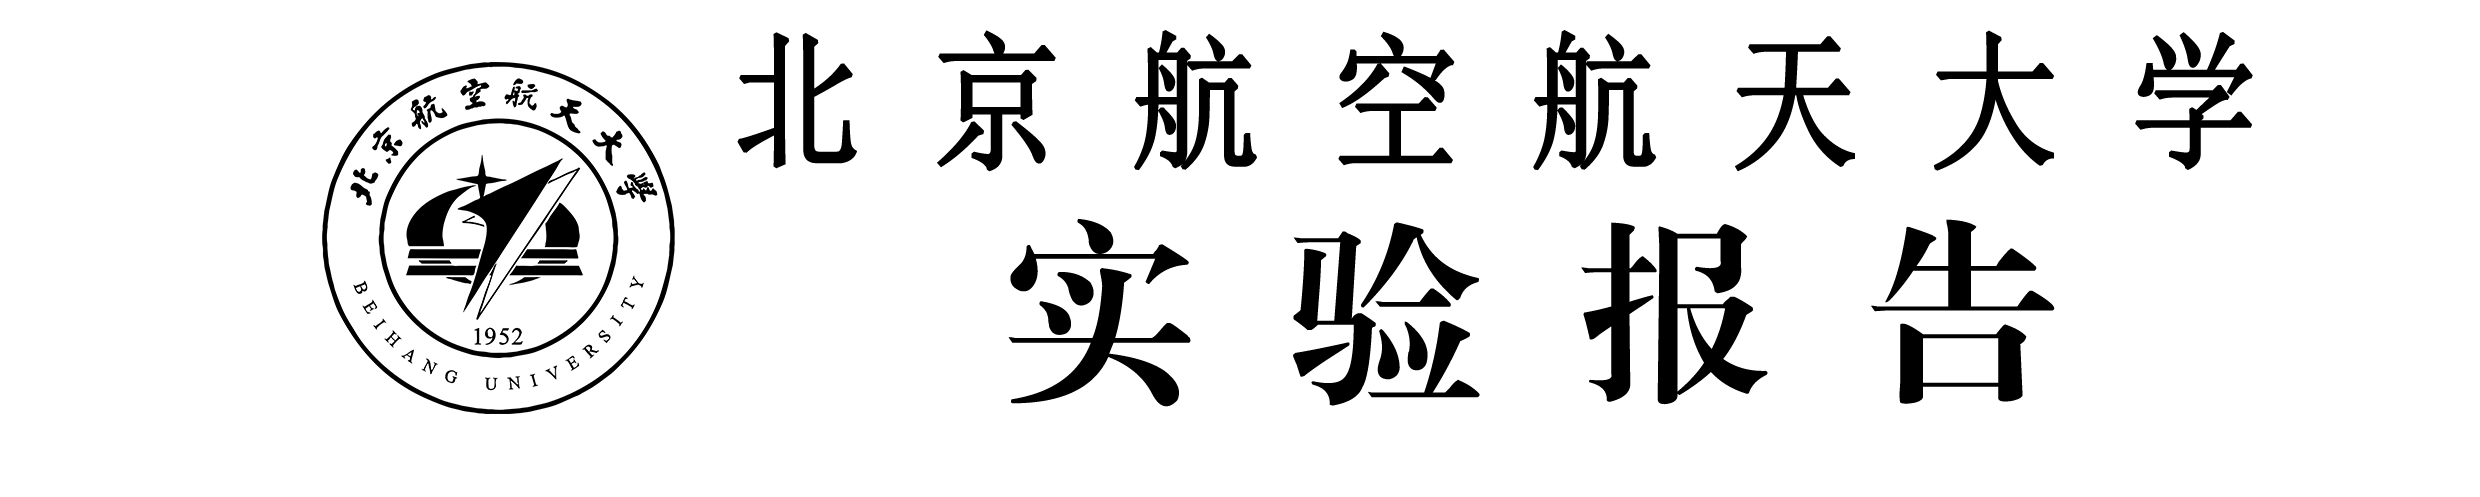
\includegraphics[width=13cm]{Image/表头.png}
\end{figure}
\begin{center}
\textbf{{\large 实验名称:\uline{          光的干涉实验1(分波面法) 钠光双棱镜干涉      }}}
\end{center}

\section*{一、 实验重点}
\begin{enumerate}
 \item 熟练掌握采用不同光源进行光路等高共轴调节的方法和技术;
 \item 用实验研究菲涅耳双棱镜干涉并测定单色光波长;
 \item 学习用钠光和其他光源进行实验时不同的调节方法。
\end{enumerate}

\section*{二、实验原理}

\subsection*{1.钠光双棱镜干涉}
菲涅耳双棱镜可以看成是有两块底面相接、棱角很小的直角棱镜合成。若置单色光源S于双棱镜的正前方,则从S射来的光束通过双棱镜的折射后,变为两束相重叠的光,
这两束光仿佛是从光源S、的两个虚像$S_1$和$S_2$射出的一样。由于$S_1$和$S_2$是两个相干光源,所以若在两束光相重叠的区域内放置一个屏,即可观察到明暗相间的干涉条纹。

\begin{wrapfigure}{r}{0.4\textwidth}
  \vspace{-20pt}
  \begin{center}
    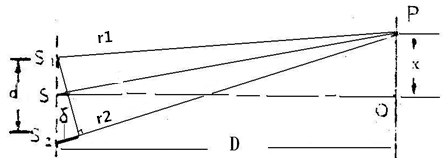
\includegraphics[width=0.48\textwidth]{Image/ExperimentScience.png}
  \end{center}
  \vspace{-20pt}
  \vspace{-10pt}
\end{wrapfigure}

如图所示,设虚光源$S_1$和$S_2$的距离是d,D是虚光源到屏的距离。
令P为屏上任意一点,$r_1$和$r_2$分别为从$S_1$和$S_2$到P点的距离,
则从$S_1$和$S_2$发出的光线到达M点的光程差是:

\begin{center}
$\bigtriangleup$L= $r_2$-$r_1$
\end{center}

令$N_1$和$N_2$分别为$S_1$和$S_2$在屏上的投影,O为${N_1}{N_2}$的中点,
并设OP=x,则从${{\bigtriangleup}{S_1}{N_1}\text{P}}$及${\bigtriangleup}{S_2}{N_2}$P得:

\begin{center}
${r_1}^2=D^2+(x-{\displaystyle\frac{d}{2}})^2$
\end{center}

\begin{center}
${r_2}^2=D^2+(x+{\displaystyle\frac{d}{2}})^2$
\end{center}

两式相减,得:
\begin{center}
${r_2}^2-{r_1}^2=2dx$
\end{center}


另外又有${r_2}^2-{r_1}^2=({r_2}-{r_1})({r_2}+{r_1})={\bigtriangleup}L({r_2}+{r_1})$。通常D较d大的很多,所以${r_2}+{r_1}$近似等于2D,因此光程差为:

\begin{center}
${\bigtriangleup}L=\displaystyle\frac{dx}{D}$
\end{center}

如果$\lambda$为光源发出的光波的波长,干涉极大和干涉极小处的光程差是:

$$\Delta L=\frac{dx}{D}=
\left\{
\begin{aligned} 
k\lambda & (k=0,\pm 1,\pm2,...) \text{明纹}\\
 \displaystyle\frac{2k+1}{2}\lambda & (k=0,\pm 1,\pm2,...) \text{暗纹}\\
\end{aligned}
\right.
$$


由上式可知,两干涉条纹之间的距离是:

\begin{center}
$\Delta x=\displaystyle\frac{D}{d}\lambda$
\end{center}

所以用实验方法测得$\bigtriangleup$x,D和d后,即可算出该单色光源的波长:

\begin{center}
$\lambda =\displaystyle\frac{d}{D}{\Delta x}$
\end{center}

\subsection*{2.钠光劳埃镜干涉}

\begin{figure}[htbp]
 \centering
  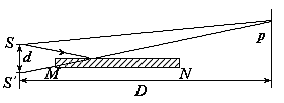
\includegraphics[width=10cm]{Image/laoai.png}
\end{figure}

劳埃镜实验是由一块普通的平板玻璃构成的反射镜实现分波前干涉。单色光源S发出的光(波长为$\lambda$)以几乎掠入射的方式在平面镜MN上发生反射,反射光可以看做是在镜中的虚像S’发出的。S和S’发出的光波在其交迭区域发生干涉,可得条纹间距为:

\begin{center}
$\Delta x=\displaystyle\frac{D}{d}\lambda$
\end{center}
   
式中d为双光源S和S’间距,D为观察屏到光源的距离。

\section*{三、实验方案}

\subsection*{1.光源的选择} 
 当双棱镜与屏的位置确定之后,干涉条纹的间距△x与光源的波长λ成正比。为了获得清晰的干涉条纹,本实验采用单色光源钠光。

\subsection*{2.测量方法}
 条纹间距${\bigtriangleup}{x}$可直接用侧位目镜测出。虚光源间距d用二次成像的方法测130得:当保持物、屏位置不变
 且间距D大于4f时,移动透镜可源在其间的两个位置成清晰的实像,一个是放大像,一个是缩小像。设b为虚光缩小像间
 距,b’为放大像间距,则两虚光源的实际距离为$d=\sqrt{b{b}'}$,其中b和b’由测微目镜读出,同时根据两次成像
 的规律,若分别测出呈缩小像和放大像时的物距S、$S^’$,则物到像屏之间的距离$D=S+S^’$。根据波长的计算公式,得波长
 和各测量值之间的关系是:
 \begin{center}
 $\lambda =\displaystyle\frac{\Delta x\sqrt{b{b}'}}{S+{S}'}$\\
 \end{center}
 
\subsection*{3.光路组成}
\begin{wrapfigure}{r}{0.4\textwidth}
  \vspace{-20pt}
  \begin{center}
    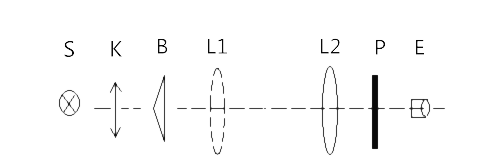
\includegraphics[width=0.48\textwidth]{Image/Instrument1071.png}
  \end{center}
  \vspace{-20pt}
  \vspace{-10pt}
\end{wrapfigure}
 具体的光路如图所示,S为半导体激光器,K为扩束镜,B为双棱镜,P为偏振片,E为测微目镜。L为测虚光源间距d所用的凸透镜,透镜位于${L_1}$位置将使虚光源${S_1}{S_2}$在目镜处成方大像,透镜位于${L_2}$处将使虚光源在目镜出成缩小像。所有光学元件都放在光具座上,光具座上附有米尺刻度读出各元件的位置。
 
\section*{四、实验仪器}
   光具座,双棱镜,测微目镜,凸透镜,扩束镜,偏振片,白屏,可调狭缝,钠光灯。
   
\section*{五、实验内容}

\subsection*{1.各光学元件的共轴调节}
\subsubsection*{1)调整狭缝与凸透镜登高共轴}
将狭缝紧贴钠灯放在光具座上,接着依次放上透镜($f\approx 20cm$)和白屏,用二次成像法使狭缝与透镜等高共轴。
\subsubsection*{2)调整测微目镜、狭缝和透镜等高共轴}
用测微目镜取代白屏,并置于距狭缝80cm位置上,进一步用二次成像法调至测微目镜叉丝与狭缝、透镜等高共轴。
\subsubsection*{3)调双棱镜或劳埃镜与其他元件共轴}
\begin{enumerate}
\item 双棱镜干涉:在狭缝与透镜之间放上双棱镜,使双棱镜到狭缝的距离约20cm,上下左右移动双棱镜并转动狭缝,直至在测微目镜中观察到等长并列(表示棱脊平行于狭缝)、等亮度(表示棱脊透过透镜光轴)的两条狭缝缩小像。
\item 劳埃镜干涉:移去透镜,在狭缝后面放上劳埃镜,通过劳埃镜目测观察双光源像,调整狭缝取向至两狭缝像相互平行,在调整劳埃镜使双光源等亮且相距较近。
\end{enumerate}

\subsection*{2.干涉条纹的调整}
\begin{enumerate}
\item 双棱镜干涉:在上述光学元件调整的基础上,移去透镜,进一步交替微调狭缝宽度和狭缝取向,反复若干次,直至通过测微目镜看到最清晰的干涉条纹为止。
\item 劳埃镜干涉:通过测微目镜进行观察,同时微微调节劳埃镜和狭缝取向,直至出现清晰的干涉条纹。
\end{enumerate}

\subsection*{3.波长的测量及数据处理}
\subsubsection*{1)测条纹间距${\bigtriangleup}$x}
连续测量20个条纹的位置${x_i}$ 。如果视场内干涉条纹没有布满,则可对测微目镜的水平位置略作调整;视场太暗可旋转偏振片调亮。
\subsubsection*{2)测量虚光源缩小像间距b及透镜物距S}
测b时应在鼓轮正反向前进时,各做一次测量。注意:i)不能改变扩束镜、双棱镜级测微目镜的位置;ii)用测微目镜读数时要消空程。
\subsubsection*{3)用上述同方法测量虚光源放大像间距b’及透镜物距S’。}

\section{六、数据处理}
\subsection{1.钠光双棱镜干涉}
\subsubsection{(1)逐差法求$\Delta x(单位:mm)$}
\begin{tabular}{|c|c|c|c|c|c|c|c|c|c|c|}
\hline 
$i$ & 1 & 2 & 3 & 4 & 5 & 6 & 7 & 8 & 9 & 10 \\ 
\hline 
$x_i$ & • & • & • & • & • & • & • & • & • & • \\ 
\hline 
$x_{i+10}$ & • & • & • & • & • & • & • & • & • & • \\ 
\hline 
$10\Delta x_i$ & • & • & • & • & • & • & • & • & • & • \\ 
\hline 
\end{tabular} 

$\bar{10\Delta x} = [10Delta x]mm$

$\therefore \Delta x = [Delat x]mm$

$u_a(10\Delta x) = \sqrt{\displaystyle\frac{\sum (10\Delta x_i-\overline{10\Delta x})^2}{10(10-1)}} = [ua10Deltax]mm$

$u_b(10\Delta x) = \displaystyle\frac{\Delta 仪}{\sqrt{3}} = \displaystyle\frac{0.005}{\sqrt{3}} = 0.00289mm$

$\therefore u(10\Delta x) = \sqrt{u_a^2(10\Delta x)+u_b^2(10\Delta x)} = [u10Delta x]mm$

$u(\Delta x) = \displaystyle\frac{u(10\Delta x)}{10} = [uDelta x]mm$

$\Delta x \pm u(\Delta x) = ([Delat x]\pm [uDelta x])mm$

\subsubsection{(2)$b$与$b'$的处理(单位:mm)}

\begin{tabular}{|c|c|c|c|c|}
\hline 
$i$ & 1左 & 1右 & 2左 & 2右 \\ 
\hline 
$b$(小像) & • & • & • & • \\ 
\hline 
$b'$(大像) & • & • & • & • \\ 
\hline 
\end{tabular} 
求得:

$\bar{b} = [b平均]mm$

$\bar{b'} = [b'平均]mm$

由成像位置判断不准带来的误差:$\Delta b = 0.025b$,$\Delta b' = 0.025b'$。

所以

$u(b) = \sqrt{(\displaystyle\frac{\Delta b}{\sqrt{3}})^2+(\displaystyle\frac{\Delta 仪}{\sqrt{3}})^2} = [ub]mm$($\Delta 仪$ 太小,忽略)

$u(b') = \sqrt{(\displaystyle\frac{\Delta b'}{\sqrt{3}})^2+(\displaystyle\frac{\Delta 仪}{\sqrt{3}})^2} = [ub']mm$($\Delta 仪$ 太小,忽略)

所以

$b \pm u(b) = ([b]\pm [ub])mm$

$b' \pm u(b') = ([b']\pm [ub'])mm$

\subsubsection{(3)$S$和$S'$的处理(单位:cm)}
\begin{tabular}{|c|c|c|c|c|c|}
\hline 
仪器 & 狭缝 & 目镜 & 双棱镜 & $L_1$(大) & $L_2$(小) \\ 
\hline 
位置 & • & • & • & • & • \\ 
\hline 
\end{tabular} 
注:表中狭缝位置经过修正

得:

$S = [狭缝] - [L2] = [S]cm$

$S' = [狭缝] - [L1] = [S']cm$

$u(S) = \sqrt{(\displaystyle\frac{\Delta S}{\sqrt{3}})^2+(\displaystyle\frac{\Delta 仪}{\sqrt{3}})^2} = [uS]mm$

$u(S') = \sqrt{(\displaystyle\frac{\Delta S'}{\sqrt{3}})^2+(\displaystyle\frac{\Delta 仪}{\sqrt{3}})^2} = [uS']mm$

\subsubsection{(4)计算$\lambda$ 并求相对误差及不确定度$u(\lambda )$}
由以上数据有:

$\lambda  = \displaystyle\frac{\Delta x\cdot \sqrt{bb'}}{S+S'} = \displaystyle\frac{[Delta x]\times \sqrt{[b][b']}}{[S]+[S']}mm = [lambda]nm$

相对误差 $\mu = \displaystyle\frac{\left | [真实值]-[lambda] \right |}{[真实值]} \times 100\% = [相对误差]$

$u(\lambda ) = \lambda \cdot \sqrt{\left [ \displaystyle\frac{u(\Delta x)}{\Delta x} \right ]^2+\left [ \displaystyle\frac{u(b)}{2b} \right ]^2+\left [ \displaystyle\frac{u(b')}{2b'} \right ]^2+\left [ \displaystyle\frac{u(S)}{S+S'} \right ]^2+\left [ \displaystyle\frac{u(S')}{S+S'} \right ]^2} = [ulambda]nm$

波长最后表述为:$\lambda \pm u(\lambda) = ([lambda]\pm [ulambda])nm$

\subsection{2.劳埃镜干涉}
\subsubsection{(1)逐差法求$\Delta x$(单位:mm)}
\begin{tabular}{|c|c|c|c|c|c|c|c|c|c|c|}
\hline 
$i$ & 1 & 2 & 3 & 4 & 5 & 6 & 7 & 8 & 9 & 10 \\ 
\hline 
$x_i$ & • & • & • & • & • & • & • & • & • & • \\ 
\hline 
$x_{i+10}$ & • & • & • & • & • & • & • & • & • & • \\ 
\hline 
$10\Delta x_i$ & • & • & • & • & • & • & • & • & • & • \\ 
\hline 
\end{tabular} 

$\bar{10\Delta x} = [10Delta x]mm$

$\therefore \Delta x = [Delat x]mm$

$u_a(10\Delta x) = \sqrt{\displaystyle\frac{\sum (10\Delta x_i-\overline{10\Delta x})^2}{10(10-1)}} = [ua10Deltax]mm$

$u_b(10\Delta x) = \displaystyle\frac{\Delta 仪}{\sqrt{3}} = \displaystyle\frac{0.005}{\sqrt{3}} = 0.00289mm$

$\therefore u(10\Delta x) = \sqrt{u_a^2(10\Delta x)+u_b^2(10\Delta x)} = [u10Delta x]mm$

$u(\Delta x) = \displaystyle\frac{u(10\Delta x)}{10} = [uDelta x]mm$

$\Delta x \pm u(\Delta x) = ([Delat x]\pm [uDelta x])mm$
\subsubsection{(2)$b$与$b'$的处理(单位:mm)}

\begin{tabular}{|c|c|c|c|c|}
\hline 
$i$ & 1左 & 1右 & 2左 & 2右 \\ 
\hline 
$b$(小像) & • & • & • & • \\ 
\hline 
$b'$(大像) & • & • & • & • \\ 
\hline 
\end{tabular} 
求得:

$\bar{b} = [b平均]mm$

$\bar{b'} = [b'平均]mm$

由成像位置判断不准带来的误差:$\Delta b = 0.025b$,$\Delta b' = 0.025b'$。

所以

$u(b) = \sqrt{(\displaystyle\frac{\Delta b}{\sqrt{3}})^2+(\displaystyle\frac{\Delta 仪}{\sqrt{3}})^2} = [ub]mm$($\Delta 仪$ 太小,忽略)

$u(b') = \sqrt{(\displaystyle\frac{\Delta b'}{\sqrt{3}})^2+(\displaystyle\frac{\Delta 仪}{\sqrt{3}})^2} = [ub']mm$($\Delta 仪$ 太小,忽略)

所以

$b \pm u(b) = ([b]\pm [ub])mm$

$b' \pm u(b') = ([b']\pm [ub'])mm$

\subsubsection{(3)$S$和$S'$的处理(单位:cm)}
\begin{tabular}{|c|c|c|c|c|c|}
\hline 
仪器 & 狭缝 & 目镜 & 双棱镜 & $L_1$(大) & $L_2$(小) \\ 
\hline 
位置 & • & • & • & • & • \\ 
\hline 
\end{tabular} 
注:表中狭缝位置经过修正

得:

$S = [狭缝] - [L2] = [S]cm$

$S' = [狭缝] - [L1] = [S']cm$

$u(S) = \sqrt{(\displaystyle\frac{\Delta S}{\sqrt{3}})^2+(\displaystyle\frac{\Delta 仪}{\sqrt{3}})^2} = [uS]mm$

$u(S') = \sqrt{(\displaystyle\frac{\Delta S'}{\sqrt{3}})^2+(\displaystyle\frac{\Delta 仪}{\sqrt{3}})^2} = [uS']mm$

\subsubsection{(4)计算$\lambda$ 并求相对误差及不确定度$u(\lambda )$}
由以上数据有:

$\lambda  = \displaystyle\frac{\Delta x\cdot \sqrt{bb'}}{S+S'} = \displaystyle\frac{[Delta x]\times \sqrt{[b][b']}}{[S]+[S']}mm = [lambda]nm$

相对误差 $\mu = \displaystyle\frac{\left | [真实值]-[lambda] \right |}{[真实值]} \times 100\% = [相对误差]$

$u(\lambda ) = \lambda \cdot \sqrt{\left [ \displaystyle\frac{u(\Delta x)}{\Delta x} \right ]^2+\left [ \displaystyle\frac{u(b)}{2b} \right ]^2+\left [ \displaystyle\frac{u(b')}{2b'} \right ]^2+\left [ \displaystyle\frac{u(S)}{S+S'} \right ]^2+\left [ \displaystyle\frac{u(S')}{S+S'} \right ]^2} = [ulambda]nm$

波长最后表述为:$\lambda \pm u(\lambda) = ([lambda]\pm [ulambda])nm$
\end{document}
